\section{Complex derivative}

\newcommand{\conj}[1]{{#1}^*}
\newcommand{\conjp}[1]{{\left(#1\right)}^*}
\def\Jacob{\bm{\mathcal{J}}}

In this section we try to describe the shape and structure of the
Jacobian over the complex scalar field, instead of what is usually done, by
considering the real and imaginary separatly. Discarding the
polarisation effects, the scalar Radio Interferometry Measurement
Equation (RIME), we can write the visibility measured on baseline
$(pq)$, at time $t$ and frequency $\nu$ as:

\def\u{u}
\def\v{v}
\def\w{w}
\def\l{l}
\def\m{m}
\def\n{n}

\begin{alignat}{2}
\label{eq:ME}
\mathrm{v}_{(pq)t\nu}=&\displaystyle\sum\limits_{d} g^{d}_{pt\nu}
.\conjp{g^{d}_{qt\nu}}.k^{d}_{(pq)t\nu}.\mathrm{s}_{d}\\
\text{with}\ k^{d}_{(pq)t\nu}=&\exp{\left(-2 i\pi
  \left(\u\l+\v\m+\w\left(\text{n}-1\right)\right)\right)}\\
\text{and}\ \n=&\sqrt{1-\l^2-\m^2}\\
\end{alignat}

\noindent with $[\u,\v,\w]^T$ is the baseline vector between antennas
$p$ and $q$ in wavelength units, and
$\vec{s}_d=[\l,\m,\n=\sqrt{1-\l^2-\m^2}]^T$ is a sky direction later
labeled as $d$. In order to compute a Jacobian, we need to choose a
derivative definition for complex numbers. If we write a complex number as $z=x+iy$, then the
Wirtinger complex derivative operator writes as:


\begin{alignat}{3}
\frac{\partial }{\partial z}&=&\frac{\partial }{\partial x}-i\frac{\partial }{\partial y}\\
\end{alignat}

\noindent where $x$ and $y$ are the real and imaginary parts
respectively. The Wirtinger has a trivial but remarquable property
that a scalar and its complex conjugate can be viewed as independent
variables, and in particular: 

\begin{alignat}{3}
\label{eq:propConj}
\frac{\partial \conj{z}}{\partial z}&=&0
\end{alignat}


Considering the sky, gain, and geometry relation given in
Eq. \ref{eq:ME}, according to the property of Wirtinger derivative of complex
conjugate (Eq. \ref{eq:propConj}), we can see that:

\begin{alignat}{2}
\frac{\partial \mathrm{v}_{(pq)t\nu}}{\partial g^{d}_{pt\nu}}=&
\conjp{g^{d}_{qt\nu}}.k^{d}_{(pq)t\nu}.\mathrm{s}_{d}\\
\text{and}\ \frac{\partial \mathrm{v}_{(pq)t\nu}}{\partial g^{d}_{qt\nu}}=&0\\
\end{alignat}


\def\JVpq{\Jacob\left\{\textbf{v}_{(pq)}\right\}}
\def\JVpq{\Jacob_{\!_{\textbf{v}_{pq}}}}
\def\JVpq{\Jacob_{{\textbf{v}_{pq}}}}
\def\JV{\Jacob\left\{\textbf{v}\right\}}
%\def\JV{\Jacob_{\!_\textbf{v}}}
\def\JV{\Jacob_{\textbf{v}}}
%\def\JVpq{\Jacob_{\textbf{V}_{(pq)}}}

We now consider the visibility vector $\textbf{v}_{(pq)}$ for all time
frequency block within a given interval. According to the definition
of Wirtinger derivative, we can write the complex Jacobian $\JVpq$ of
$\textbf{V}_{(pq)}$ of size $[(n_t n_{\nu})\times (n_a n_d)]$, where
$n_t$, $n_{\nu}$, $n_a$, and $n_d$ are the number of time, frequency,
antenna and directions. Each cell of
$\JVpq$ can be written by taking a line corresponding to the
measurement at $(t\nu)$, and a column $i=d+a.n_d$ (for given antenna $a$ and direction $d$)
corresponds to the derivative against $g^{d}_{a}$. We have:


%% \begin{alignat}{2}
%% \mathcal{J}\left(\textbf{V}_{(pq)}\right)=&caca\\
%% \end{alignat}


\begin{alignat}{2}
\label{eq:Jpq}
\left[\JVpq\right]_{t\nu,i}=&
\begin{cases}
\conjp{g^{d}_{qt\nu}}.k^{d}_{(pq)t\nu}.\mathrm{s}_{d}\text{ for }a=p\\
0\ \text{otherwise}
\end{cases}
\end{alignat}

\noindent We can see that non-zero columns are the ones
corresponding to all direction for antenna $p$. The Jacobian for all
baselines is written in a similar way, by superposing the
$\JVpq$ for all $(pq)$ pairs as follows:



\begin{alignat}{2}
\label{eq:J}
\JV=&
\begin{bmatrix} 
\vdots \\ 
\JVpq\\ 
\vdots \\ 
\end{bmatrix}
\end{alignat}

\noindent which have size $[(n_{bl} n_t n_{\nu})\times (n_a n_d)]$,
where $n_{bl}$ is the number of baselines and is typically
$n_{bl}=n_a(n_a-1)/2$. Although it has large dimensions, $\JV$ is
sparse.


\begin{figure*}[ht!]
\begin{center}
%\hspace*{-1.3cm}
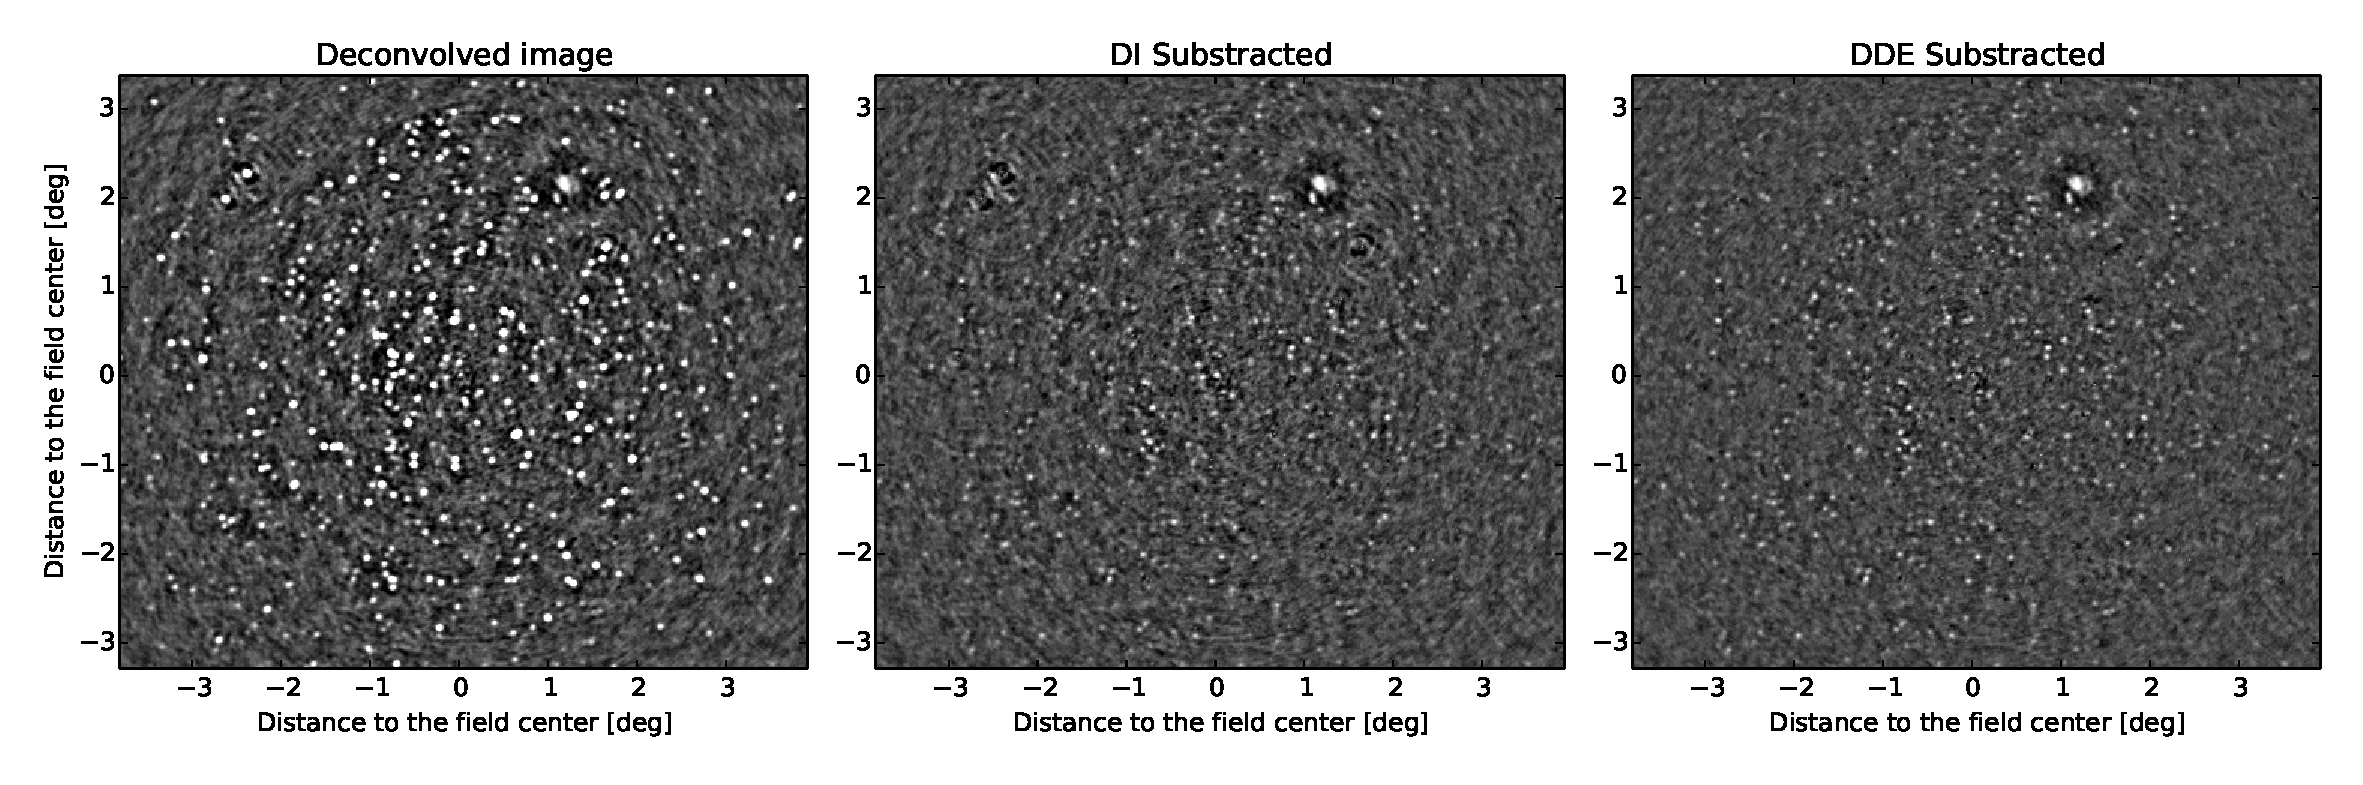
\includegraphics[width=17cm]{resid.eps}
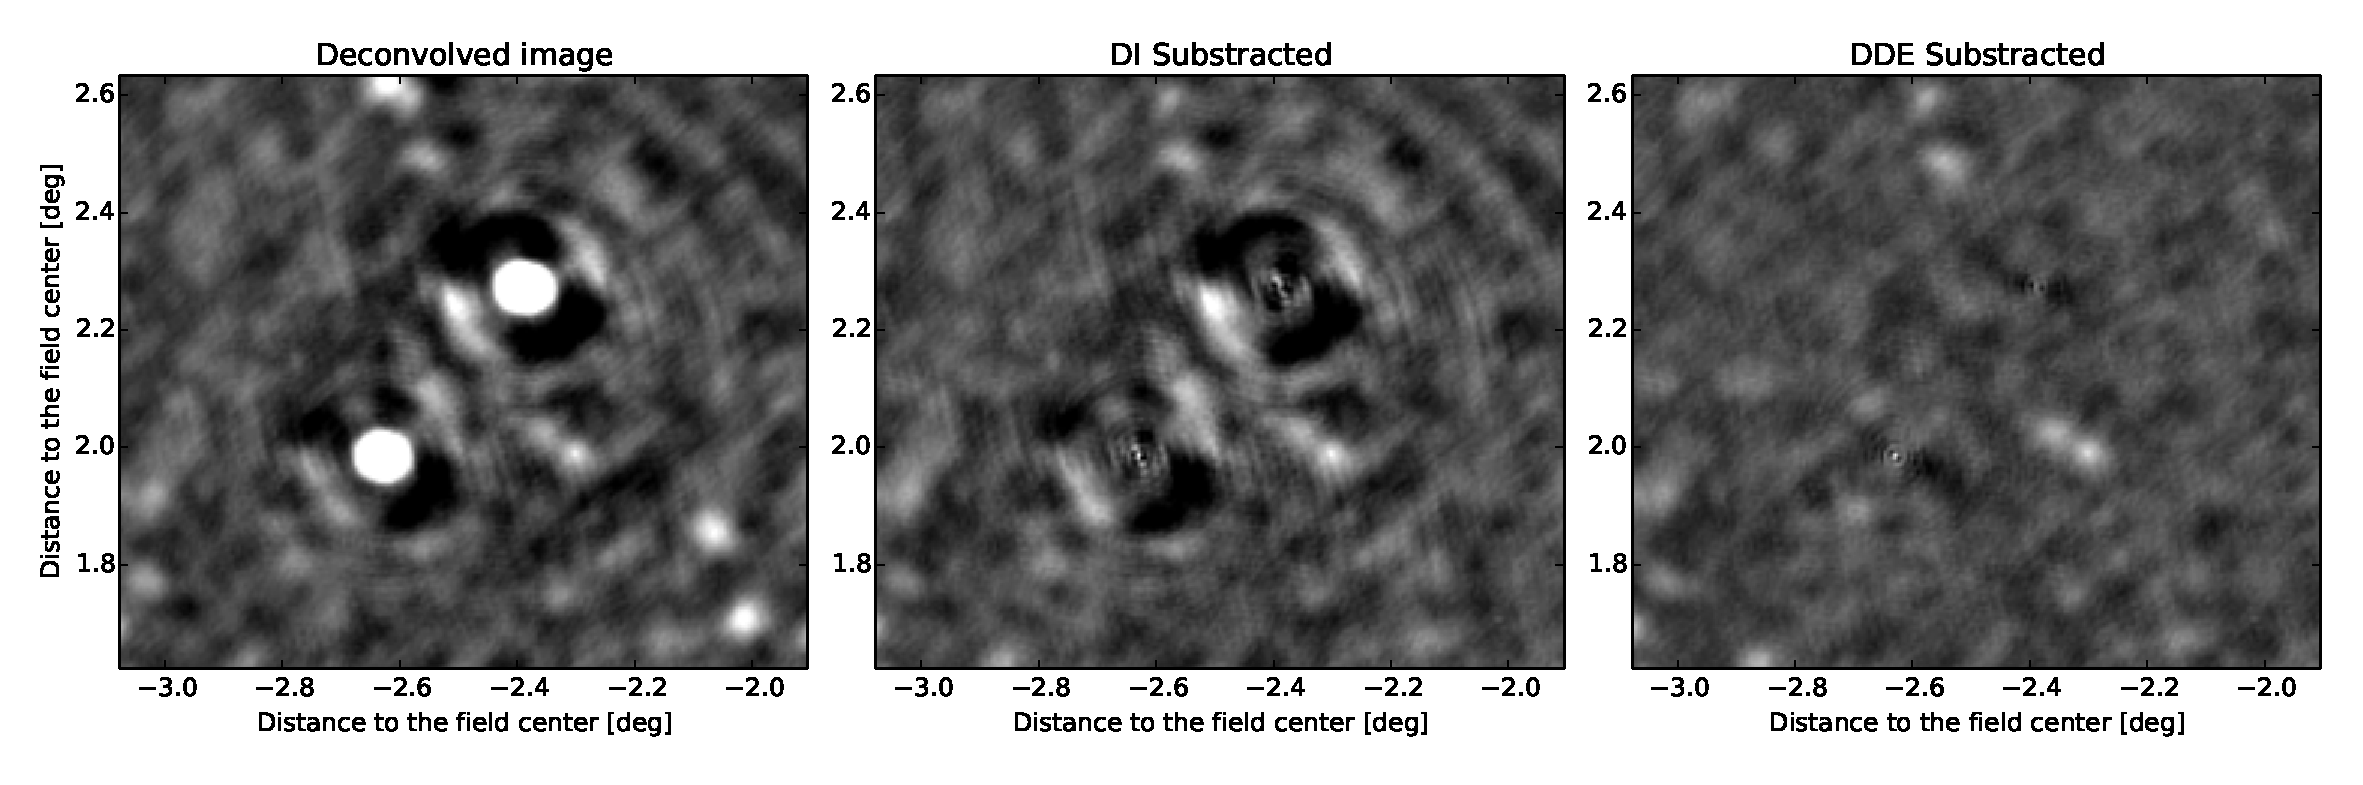
\includegraphics[width=17cm]{residZoom.eps}
\caption{\label{fig:resid} This figure shows compares the image
  (left), the residuals data after simple skymodel substraction
  (center), and the residuals data after substracting the
  sky model corrupted by the direction-dependent solution (right).}
\end{center}
\end{figure*}

